\documentclass[conference]{ieeeconf}
%\documentclass{article}

\usepackage{graphicx}
%\usepackage{natbib}


% AM PIN 190870
%The registration of Amilcar Malave (PIN 190870) was successfully completed
%A notification was successfully sent to amilcar.malave1997@gmail.com

%The registration of Emily Valera (PIN 190875) was successfully completed
%A notification was successfully sent to e.rose.valera@gmail.com

% EK 18591 


%\setcitestyle{numbers,square}

\title{Modulation of Human Brain Functional Connectivity with Transcranial Focused Ultrasound Stimulation}

\author{Amilcar Malave$^{1}$, Emily Valera$^{2}$, Elisa Konofagou$^{3}$, Jacek P. Dmochowski$^{2}$
\thanks{$^{1}$Graduate School of Education, Stanford University, CA, USA.}
\thanks{$^{2}$Department of Biomedical Engineering, City College of New York, NY, USA.}
\thanks{$^{3}$Department of Biomedical Engineering, Columbia University, NY, USA.}}

\begin{document}

\maketitle

\begin{abstract} \noindent
Transcranial focused ultrasound stimulation (tFUS) is being increasingly investigated as a non-invasive approach to interrogate brain circuits and treat psychiatric disorders marked by aberrant brain activity. However, the mechanisms of tFUS, as well as its effects on large-scale brain networks, remain unclear. Here, we asked whether tFUS can reliably modulate functional connectivity (FC) with a deep brain region: the subgenual anterior cingulate cortex (sgACC), a clinically relevant area implicated in mood disorders. Using functional magnetic resonance imaging (fMRI), we recorded blood-oxygen-level dependent (BOLD) activity before, during, and after 5 minutes of tFUS targeting the sgACC. Relative to sham stimulation, we found a statistically significant increase in FC with the target both during and immediately after sonication. The increase manifested as a slow increase that was observed in approximately 80\% of the sgACC's connections, suggesting enhanced integration of the sgACC into large-scale networks. These findings support the feasibility of tFUS as a tool for modulating activity in deep brain regions with potential therapeutic applications. 
\end{abstract}

\section{Introduction} \noindent
Transcranial focused ultrasound stimulation (tFUS) is being increasingly investigated as a non-invasive neuromodulation technique capable of transiently modulating brain activity with high spatial resolution \cite{Naor2016-wz,blackmore2019mechanisms}. Unlike its electromagnetic counterparts -- transcranial magnetic stimulation (TMS) and transcranial direct current stimulation (tDCS) --  tFUS can reach deep brain structures while preserving focal targeting, making it an attractive tool for both basic neuroscience and clinical applications. Pioneering studies by Tyler et al. \cite{Tyler2008-zs}, Tufail et al, \cite{Tufail2010-jd} and Legon et al. \cite{legon2014transcranial} demonstrated the feasibility of ultrasonic neuromodulation of \emph{in vitro}, small animal and human models, respectively, laying the foundation for subsequent investigations into its underlying mechanisms and functional effects. 

Nevertheless, the mechanisms by which tFUS influences neural activity remain unclear and represent an area of active investigation \cite{Blackmore2019-zo,kamimura2020ultrasound,dell2022current}. Several hypotheses have been proposed, including mechanical effects on mechanosensitive ion channels, alterations in membrane capacitance, flexoelectricity, and astrocytic modulation. Identifying the genuine mechanisms is crucial to the desired ability to regulate neural activity in a directional manner: increasing (or decreasing) excitation (or inhibition) in the targeted region. 

A growing body of literature has investigated the effects of tFUS on large-scale brain networks, including its impact on functional connectivity (FC) as measured by functional magnetic resonance imaging (fMRI). FC refers to the correlation of neural signals between pairs of brain regions, most commonly measured with the blood-oxygen-level dependent (BOLD) signal. BOLD FC serves as a robust biomarker of brain state and clinical phenotype \cite{rogers2007assessing, van2010exploring}. Past studies have reported both increases and decreases in functional connectivity following tFUS, suggesting that its effects depend on the nature of the target, ultrasonic waveform, and experimental context. Chou et al. \cite{chou2024transcranial} and Yaakub et al. \cite{yaakub2023transcranial} demonstrated that tFUS can enhance connectivity in targeted networks, whereas other studies have reported reductions in connectivity \cite{todd2018focused,meng2019resting,sanguinetti2020transcranial,zhang2021low,kuhn2023transcranial,lord2024transcranial}. 

The present study aims to investigate whether tFUS can reliably modulate the activity of a clinically relevant deep brain structure, the subgenual anterior cingulate cortex (sgACC), which plays a central role in mood regulation and affective processing \cite{drevets2008subgenual}, with a particular relevance to major depression \cite{greicius2007resting}. We conducted a within-subject, sham-controlled study in 16 healthy adults that combined tFUS with fMRI BOLD. Subjects were stimulated inside the MRI scanner such that we could evaluate the effects of sonication on our primary dependent variable, namely the FC with the targeted sgACC. 

Despite the modest sample size of our cohort, we were indeed able to resolve a statistically significant increase in FC with the sgACC region. Interestingly, the increase was more pronounced in the period following tFUS, hinting at the capability of tFUS to produce changes that outlast the period of sonication. These results suggest that tFUS may promote the integration of the sgACC into large-scale brain networks.
By elucidating the impact of tFUS on FC, this study contributes to the growing understanding of ultrasound neuromodulation and its translational potential for clinical applications. 

\begin{figure}
    \centering
    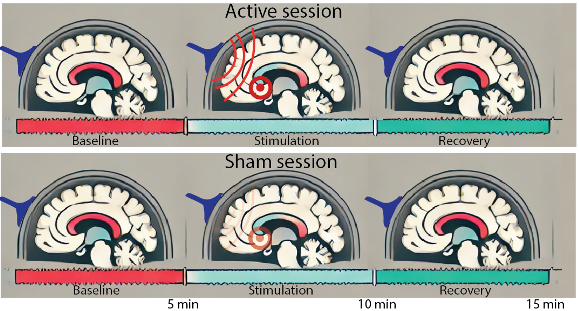
\includegraphics[width=\linewidth]{exp_design.png}
    \caption{Experimental design: subjects participated in two experimental sessions spaced two weeks apart. Each session consisted of a continuous, 15 minute fMRI BOLD scan where either active or sham tFUS targeting the sgACC was applied in the middle 5 minute segment. The order of the sessions was randomized and counterbalanced across subjects. }
    \label{fig:exp}
\end{figure}

\section*{Methods} \noindent
\subsection*{Participants}
Sixteen healthy adults (7 females; age 26 $\pm$ 7 years, mean $\pm$ standard deviation) participated in a within-subjects study consisting of two sessions employing active and sham tFUS, respectively (Fig \ref{fig:exp}). Sessions were spaced two weeks apart to ensure sufficient washout of effects. The order of the sessions was randomized and counterbalanced across the cohort. Experimental procedures were approved by the Institutional Review Board of the City University of New York, and subjects provided written informed consent prior to participation. 

\subsection*{tFUS Parameters}
Transcranial focused ultrasound stimulation (tFUS) was delivered at 500 kHz with a circular transducer (Sonic Concepts CTX-500) driven by an integrated signal generator and amplifier (Sonic Concepts NeuroFUS). The waveform was pulsed with a repetition frequency (PRF) of 40 Hz and a duty cycle of 30\%. Sonication duration was 20 s, with a 40 s interval between successive sonications. All subjects received a total of 5 sonications. Acoustic intensity was measured in a water tank under free-field conditions with a calibrated hydrophone (ONDA corporation) as $I_{\mathrm{spta}} = 667$ mW/cm$^2$. 

The transducer positioning relied on a computational procedure to identify the subject-specific optimal scalp location for targeting the sgACC. To that end, the subject’s anatomical MRI was employed to exhaustively search across a broad range of discretized scalp positions to identify the coordinates on the forehead (frontal pole region) whose normal vector most closely intersected the right sgACC. This resulted in a variable distance to the target across subjects (approximately 5-6 cm), which was accommodated by the tFUS system’s steering of the focal depth. The transducer was fixed to the subject's scalp using an elastic headband. 

\subsection*{MRI and fMRI}
Imaging was performed at 3 T with a Siemens Magnetom Prisma. Structural images were acquired with a T1-weighted MPRAGE sequence employing isotropic 0.8 mm voxels. Resting-state functional BOLD scans were acquired with a multi-echo echo-planar imaging (EPI) sequence (2 mm isotropic voxels, TR=1000 ms, TE=37 ms, flip angle=52 degrees). Subjects were instructed to rest but stay awake and to not think about anything in particular.

The duration of the BOLD acquisition was 15 minutes (900 TRs). During the active tFUS session, sonication commenced at 300 s; no sonication was applied during the sham session. Subjects did not report perceptions of tFUS after the conclusion of their two sessions. 

fMRI data was preprocessed with \emph{fMRIPrep} \cite{fmriprep1,fmriprep2,nipype1,nipype2}. T1w images were corrected for intensity non-uniformity (INU)
with \texttt{N4BiasFieldCorrection} \cite{n4}, distributed with ANTs \cite{ants}, and used as the T1w-reference
throughout the workflow. The T1w-reference was then skull-stripped with
a \emph{Nipype} implementation of the \texttt{antsBrainExtraction.sh}
workflow (from ANTs), using OASIS30ANTs as the target template. Brain tissue
segmentation of cerebrospinal fluid (CSF), white-matter (WM) and
gray-matter (GM) was performed on the brain-extracted T1w using
\texttt{fast} \cite{fsl_fast}. Brain
surfaces were reconstructed using \texttt{recon-all} \cite{fs_reconall}, and the brain mask estimated
previously was refined with a custom variation of the method to
reconcile ANTs-derived and FreeSurfer-derived segmentations of the
cortical gray-matter of Mindboggle
\cite{mindboggle}. Volume-based spatial
normalization to one standard space (MNI152NLin2009cAsym) was performed
through nonlinear registration with \texttt{antsRegistration} (ANTs
2.5.1), using brain-extracted versions of both the T1w reference and the T1w
template. The ICBM 152 Nonlinear Asymmetrical
template version 2009c \cite{mni152nlin2009casym} was employed for spatial
normalization.

\subsubsection*{BOLD preprocessing} 
First, a reference
volume was generated, using a custom methodology of \emph{fMRIPrep}, for
use in head motion correction. Head-motion parameters with respect to
the BOLD reference (transformation matrices, and six corresponding
rotation and translation parameters) are estimated before any
spatiotemporal filtering using \texttt{mcflirt} \cite{mcflirt}. The BOLD reference was then co-registered to the
T1w reference using \texttt{bbregister} (FreeSurfer) which implements
boundary-based registration \cite{bbr}. Co-registration was configured
with six degrees of freedom. Several confounding time-series were
calculated based on the preprocessed BOLD: framewise displacement
(FD), DVARS and three region-wise global signals. FD was computed using
two formulations following Power (absolute sum of relative motions,
\cite{power_fd_dvars}) and Jenkinson (relative root mean square
displacement between affines, \cite{mcflirt}). FD and DVARS are
calculated for each functional run, both using their implementations in
\emph{Nipype} \cite{power_fd_dvars}.
The three global signals are extracted within the CSF, the WM, and the
whole-brain masks. Additionally, a set of physiological regressors were
extracted to allow for component-based noise correction
\cite{compcor}. Principal components are estimated
after high-pass filtering the preprocessed BOLD time-series
(using a discrete cosine filter with 128s cut-off) for the two
\emph{CompCor} variants: temporal (tCompCor) and anatomical (aCompCor).
tCompCor components are then calculated from the top 2\% variable voxels
within the brain mask. For aCompCor, three probabilistic masks (CSF, WM
and combined CSF+WM) are generated in anatomical space. Finally,
these masks are resampled into BOLD space and binarized by thresholding
at 0.99. Components are also
calculated separately within the WM and CSF masks. For each CompCor
decomposition, the \emph{k} components with the largest singular values
are retained, such that the retained components' time series are
sufficient to explain 50 percent of variance across the nuisance mask
(CSF, WM, combined, or temporal). The remaining components are dropped
from consideration. The head-motion estimates calculated in the
correction step were also placed within the corresponding confounds
file. The confound time series derived from head motion estimates and
global signals were expanded with the inclusion of temporal derivatives
and quadratic terms for each \cite{confounds_satterthwaite_2013}.
Frames that exceeded a threshold of 0.5 mm FD or 1.5 standardized DVARS
were annotated as motion outliers. Additional nuisance timeseries are
calculated by means of principal components analysis of the signal found
within a thin band of voxels around the edge of the
brain, as proposed by \cite{patriat_improved_2017}. Volumetric
resamplings were performed using \texttt{nitransforms}, configured with
cubic B-spline interpolation.

\subsection*{Statistical testing}
To test for significant differences in FC between the active and sham conditions, we employed paired, two-tailed t-tests on differences of FC (Pearson correlation coefficient) between either the baseline (initial 5 minutes) and sonication (middle 5 minutes), or between baseline and post-sonication (final 5 minutes) periods. All tests utilized a sample size of $n=16$ subjects. 

\section*{Results} \noindent
We first considered brain-wide FC changes observed during and immediately after sonication. Our primary hypothesis pertained to enhanced connectivity with the sonicated region (i.e., sgACC), and we did not expect to observe changes in connectivity between pairs of unsonicated regions. To our surprise, we found mild increases of 7.4\% during active sonication (compared to a decrease of 3.0\% during sham; relative to baseline, computed on pairs of subject-averaged FC changes observed across all $n_{\mathrm{pairs}}=1024 \times 1023/2=523776$ pairs of unique brain regions), and 15.3\% immediately after active sonication (compared to an increase of 3.8\% immediately after sham). These increases are evident in rightward shifts of the histogram of FC changes during and after tFUS (Fig \ref{fig:global}a and b, respectively).

\begin{figure*}
       \centering
    
\includegraphics[width=1.0\linewidth]{fc_diff_hist.png}
    \caption{Brain-wide functional connectivity (FC) changes observed during and immediately after sonication. {\bf(a)} Histogram of FC differences between baseline and sonication periods, shown separately for active and sham conditions. Each sample was formed as the across-subject average ($n=16$) of the FC between a unique pair of brain regions. A slight increase is evident in the active distribution's rightward shift. The mean increase was 7.3\% during active sonication, compared to a 3.0\% decrease during sham. {\bf(b)} Same as (a) but now shown for the difference between baseline and post-sonication periods. An increase of 15.3\% was observed during active tFUS, compared to a 3.8\% increase during sham. }
    \label{fig:global} 
\end{figure*}

%During tFUS, active stimulation led to a 7.37\% change in functional connectivity, while sham stimulation led to a -3.01\% change. After tFUS, active stimulation led to a 15.28\% change in functional connectivity, while sham stimulation led to a 3.81\% change.

Critically, we then probed changes in connectivity between the sonicated sgACC and other brain regions. We first computed total connectivity, taken here as the mean of the FC between sgACC and the 1023 remaining ROIs. The resulting measure showed a statistically significant increase both during and immediately after sonication (Fig \ref{fig:total}; during sonication: $t=2.34$, $p=0.034$, $n=16$, paired two-tailed t-test; (b) after sonication: $t=2.44$, $p=0.028$). 

Despite the fact that the absolute change in FC was modest (0.03 and 0.06 during and after active tFUS), these represented substantial increases from baseline connectivity: 50.6\% during and 91.3\% after active stimulation, compared to reductions of 21.4\% and 14.4\% for sham stimulation. Thus, tFUS produced significant increases in FC from initially modest baseline levels. We also point out that the \emph{variability} in FC change was markedly lower for active stimulation: 0.05 during and 0.07 immediately after active tFUS, compared to 0.09 and 0.12 for sham tFUS. 

\begin{figure}
       \centering
\includegraphics[width=1.0\linewidth]{fc_change_barplot.png}
    \caption{FC with the sonicated region increases during tFUS. Horizontal axis depicts the condition (active or sham stimulation), while the vertical axis depicts the change in FC between the baseline and sonication periods. Each marker represents one subject. A significant increase in FC was resolved during active stimulation relative to sham ($t=2.34$, $p=0.034$, $n=16$, paired two-tailed t-test. Bars represent the mean. Error bars depict the sem. }
    \label{fig:total} 
\end{figure}

\begin{figure}
       \centering
\includegraphics[width=1.0\linewidth]{fc_change_barplot_post.png}
    \caption{FC with the sonicated region increases immediately after tFUS. Same as Fig \ref{fig:total} but now shown for the period following sonication. A significant increase relative to sham was again resolved ($t=2.44$, $p=0.028$, $n=16$, paired two-tailed t-test)}
    \label{fig:total_post} 
\end{figure}

As the total connectivity is an aggregate over all connections, we next considered the FC changes separately for each ROI. For each of the 1023 connections with the targeted sgACC, we averaged the change in FC across subjects. This revealed a clear trend of generally increased connectivity during and after active tFUS but not for sham sonication (Fig \ref{fig:total_separate}. During active tFUS, 79\% of sgACC connections showed increases in FC compared to 34\% during sham stimulation. Similarly, 87\% of sgACC connections were strengthened immediately following active tFUS, whereas only 42\% were strengthened following sham tFUS. This is evidential of the observed increases in connectivity representing genuine neuromodulatory effects versus spontaneous changes related to endogenous neural dynamics. 

\begin{figure*}
       \centering

\includegraphics[width=1.0\linewidth]{sgACC_fc_change.png}
    \caption{Effects of tFUS on FC at each conencting ROI. {\bf(a)} The horizontal axis depicts the change in FC during either active (blue) or sham (orange) tFUS relative to baseline. Vertical axis spans the 1023 ROIs distinct from the sonicated sgACC. 79\% of connections strengthened during active tFUS, compared to 34\% during sham stimulation. {\bf(b)} Same as (a) but now shown for the period following tFUS. 87\% of connections showed increased FC after active sonication, compared to 42\% after sham tFUS.}
    \label{fig:total_separate} 
\end{figure*}

In order to probe the dynamics of connectivity throughout the experiment, we computed FC across sliding windows of 20 s duration. Computed in this manner, the resulting measure is termed dynamic FC (dFC) in the literature. The limited sample inherent to time-resolved BOLD measures led to substantial variability in both sham and active dFC traces. Nevertheless, examination of the dynamics exhibits a slow increase during and after active tFUS that exceeded the corresponding trend during and after sham tFUS (Fig \ref{fig:dFc}; 
regression coefficients of BOLD FC onto time for active tFUS during sonication: slope = $7.0 \times 10^{-5}$, 
intercept = $0.051$; 
sham tFUS: slope = $4.4 \times 10^{-5}$, 
intercept = $0.047$; 
regression coefficients of BOLD FC onto time for active tFUS after sonication: slope = $1.4 \times 10^{-4}$, 
intercept = $1.3 \times 10^{-3}$; 
sham tFUS: slope = $3.6 \times 10^{-6}$, 
intercept = $0.094$). 

\begin{figure*}
       \centering
\includegraphics[width=1.0\linewidth]{fc_timecourse.png}
    \caption{Dynamics of FC before, during, and after active and sham tFUS. (a) Horizontal axis depicts time, with sham sonication applied in the middle 300 s of the recording. Vertical axis depicts dFC, computed along windows with a 20 s (equivalent to 20 TRs or samples here) duration. (b) Same as (a) but now shown for active tFUS. }
    \label{fig:dFc} 
\end{figure*}

\section{Discussion} \noindent
The observed increase in connectivity between the sgACC and widespread brain regions during and after tFUS provides evidence that low-intensity ultrasound can enhance neural integration within large-scale brain networks. Our results are consistent with previous findings that have demonstrated tFUS-induced increases in FC in human and primate models \cite{Verhagen2019-ae,yaakub2023transcranial,chou2024transcranial}, while deviating from earlier studies that reported reduced FC with sonication \cite{todd2018focused,meng2019resting,sanguinetti2020transcranial,zhang2021low,kuhn2023transcranial,lord2024transcranial}. The location and function of the present target, namely the sgACC, as well as differences in the intensity, duration, and ultrasonic waveform, are potential drivers of the discrepancies in outcome between tFUS studies of FC. Indeed, a central challenge in tFUS is to identify the relationship between the tFUS parameters, the region of sonication, and the subsequent effects on neural dynamics. Elucidating these relationships is complicated by the brain's dense interconnectedness: when modulating a brain area with tFUS, it is possible that an indirect (synaptic) modulation of its connected regions will also be produced. This is a potential explanation of our finding of global FC increases, particularly following sonication (Fig \ref{fig:global}). By perturbing the sgACC, downstream modulation in the connectivity between pairs of non-sonicated regions may have ensued. 

A critical aspect of our findings is the sustained enhancement in FC following stimulation. This aligns with previous studies \cite{Verhagen2019-ae,zhang2023excitatory,yaakub2023transcranial} reporting prolonged neuromodulatory effects following tFUS, potentially due to neuroplastic mechanisms \cite{bault2024early}. It has been proposed that tFUS may influence neural activity through multiple pathways, including the activation of mechanosensitive ion channels \cite{kubanek2016ultrasound}, alterations in membrane capacitance \cite{krasovitski2011intramembrane}, and astrocytic involvement \cite{yang2015enhancement}. The slow increase in connectivity over time observed in this study suggests that tFUS may induce synaptic modifications, possibly involving long-term potentiation (LTP)-like processes. This interpretation is bolstered by the fact that the effects on connectivity were larger in the period after sonication. Thus, any acute effects of tFUS on the membrane potential of the stimulated region likely led to a slower, more chronic effect on network activity. 


%The sgACC is a crucial node in networks associated with affect regulation, including the default mode network (DMN) and limbic circuits, and its connectivity has been implicated in the pathophysiology of mood disorders \cite{drevets2008subgenual, greicius2007resting}.



%While previous studies have demonstrated bidirectional effects of tFUS on FC, with some studies reporting connectivity decreases \cite{zhang2021focused, meng2019ultrasound}, our findings highlight a region-dependent response. The sgACC’s strong involvement in affective processing suggests that its stimulation may preferentially enhance connectivity in networks that regulate mood and autonomic function. Additionally, our results provide further support for tFUS as a viable tool for non-invasively modulating deep brain regions, a capability that has remained elusive for many other neuromodulatory techniques \cite{legon2014transcranial, tyler2008ultrasound}.

%The clinical implications of these findings warrant further exploration. Given the well-established role of the sgACC in major depressive disorder (MDD) \cite{greicius2007resting}, tFUS may represent a potential therapeutic approach for mood disorders. Indeed, previous work has suggested that modulating sgACC activity via other neuromodulatory approaches, such as deep brain stimulation (DBS), can lead to significant improvements in depressive symptoms \cite{drevets2008subgenual}. Unlike DBS, however, tFUS is entirely non-invasive, making it a more accessible alternative with fewer associated risks.

%Future studies should address several key questions raised by this work. First, the precise neurophysiological mechanisms underlying tFUS-induced FC changes require further elucidation, potentially through concurrent electrophysiological recordings \cite{naor2016ultrasonic}. Second, longitudinal studies in both healthy and clinical populations are needed to determine whether repeated tFUS sessions yield cumulative or lasting effects on network dynamics. Finally, the parameter space for tFUS stimulation, including intensity, frequency, and duty cycle, should be further optimized to maximize its neuromodulatory efficacy.

Our study is not without limitations. Firstly, the BOLD signal is challenging to interpret due to the complex biophysics that give rise to its generation \cite{buxton2013physics}. In particular, neurovascular coupling is largely agnostic to excitatory versus inhibitory neurotransmission \cite{logothetis2008we}, meaning that it is challenging to infer the effect of tFUS on cortical excitability and the overall direction of the change in neural activity. Our employment of FC as the dependent variable further highlights this problem, as an increase in connectivity may be coupled with increases or decreases of the signals comprising the pair of signals being correlated. Alternative forms of MRI such as Magnetic Resonance Spectroscopy (MRS) \cite{yaakub2023transcranial} could permit a clearer understanding of the relative effects of tFUS on excitation and inhibition. Similarly, the utilization of concurrent electrophysiological recordings \cite{kim2023transcranial,mueller2014transcranial,kim2022neuromodulation,lee2016transcranial,min2011focused} may afford more direct insight into how sonication modulates neural activity. Secondly, our study employed a cohort of healthy adult subjects lacking a clinical diagnosis of major depression. As such, it is unclear whether the modulation of sgACC connectivity found here translates to brains whose activity is dysregulated by an affective disorder. Notably, the level of baseline sgACC activity was fairly modest in our data. Future studies investigating tFUS in clinical populations with aberrant sgACC dynamics are motivated by the present study. 

\section*{Conclusions} \noindent
In summary, this study has provided evidence for the ability of tFUS to enhance FC in deep brain regions of the healthy human brain. The present data indicates that ultrasound produces changes in brain connectivity that persist beyond the period of sonication. More broadly, our results point to the potential of ultrasonic neuromodulation as a non-invasive tool for interrogating neural circuits and developing non-pharmacological approaches to combating psychiatric disorders.

\section{Acknowledgments} \noindent
The authors thank Ahmed ``Duke'' Shereen (CUNY Advanced Science Research Center) for his help with the development of the imaging experiments.


\bibliographystyle{ieeetr}
\bibliography{references}


\end{document}
\begin{thebibliography}{49}
\providecommand{\natexlab}[1]{#1}
\providecommand{\url}[1]{\texttt{#1}}
\expandafter\ifx\csname urlstyle\endcsname\relax
  \providecommand{\doi}[1]{doi: #1}\else
  \providecommand{\doi}{doi: \begingroup \urlstyle{rm}\Url}\fi

\bibitem[Avants et~al.(2008)Avants, Epstein, Grossman, and Gee]{ants}
B.~Avants, C.~Epstein, M.~Grossman, and J.~Gee.
\newblock Symmetric diffeomorphic image registration with cross-correlation: Evaluating automated labeling of elderly and neurodegenerative brain.
\newblock \emph{Medical Image Analysis}, 12\penalty0 (1):\penalty0 26--41, 2008.
\newblock ISSN 1361-8415.
\newblock \doi{10.1016/j.media.2007.06.004}.
\newblock URL \url{https://www.sciencedirect.com/science/article/pii/S1361841507000606}.

\bibitem[Bault et~al.(2024)Bault, Yaakub, and Fouragnan]{bault2024early}
N.~Bault, S.~N. Yaakub, and E.~Fouragnan.
\newblock Early-phase neuroplasticity induced by offline transcranial ultrasound stimulation in primates.
\newblock \emph{Current Opinion in Behavioral Sciences}, 56:\penalty0 101370, 2024.

\bibitem[Behzadi et~al.(2007)Behzadi, Restom, Liau, and Liu]{compcor}
Y.~Behzadi, K.~Restom, J.~Liau, and T.~T. Liu.
\newblock A component based noise correction method ({CompCor}) for {BOLD} and perfusion based fmri.
\newblock \emph{NeuroImage}, 37\penalty0 (1):\penalty0 90--101, 2007.
\newblock ISSN 1053-8119.
\newblock \doi{10.1016/j.neuroimage.2007.04.042}.
\newblock URL \url{https://www.sciencedirect.com/science/article/pii/S1053811907003837}.

\bibitem[Blackmore et~al.(2019{\natexlab{a}})Blackmore, Shrivastava, Sallet, Butler, and Cleveland]{Blackmore2019-zo}
J.~Blackmore, S.~Shrivastava, J.~Sallet, C.~R. Butler, and R.~O. Cleveland.
\newblock Ultrasound neuromodulation: A review of results, mechanisms and safety.
\newblock \emph{Ultrasound Med. Biol.}, 45\penalty0 (7):\penalty0 1509--1536, July 2019{\natexlab{a}}.

\bibitem[Blackmore et~al.(2019{\natexlab{b}})]{blackmore2019mechanisms}
J.~Blackmore et~al.
\newblock Mechanisms of ultrasound neuromodulation.
\newblock \emph{Ultrasound Med Biol}, 2019{\natexlab{b}}.

\bibitem[Buxton(2013)]{buxton2013physics}
R.~B. Buxton.
\newblock The physics of functional magnetic resonance imaging (fmri).
\newblock \emph{Reports on Progress in Physics}, 76\penalty0 (9):\penalty0 096601, 2013.

\bibitem[Chou et~al.(2024)Chou, Deckersbach, Guerin, Wong, Borron, Kanabar, Hayden, Long, Daneshzand, Pace-Schott, et~al.]{chou2024transcranial}
T.~Chou, T.~Deckersbach, B.~Guerin, K.~S. Wong, B.~M. Borron, A.~Kanabar, A.~N. Hayden, M.~P. Long, M.~Daneshzand, E.~F. Pace-Schott, et~al.
\newblock Transcranial focused ultrasound of the amygdala modulates fear network activation and connectivity.
\newblock \emph{Brain Stimulation}, 17\penalty0 (2):\penalty0 312--320, 2024.

\bibitem[Dale et~al.(1999)Dale, Fischl, and Sereno]{fs_reconall}
A.~M. Dale, B.~Fischl, and M.~I. Sereno.
\newblock Cortical surface-based analysis: I. segmentation and surface reconstruction.
\newblock \emph{NeuroImage}, 9\penalty0 (2):\penalty0 179--194, 1999.
\newblock ISSN 1053-8119.
\newblock \doi{10.1006/nimg.1998.0395}.
\newblock URL \url{https://www.sciencedirect.com/science/article/pii/S1053811998903950}.

\bibitem[Dell'Italia et~al.(2022)Dell'Italia, Sanguinetti, Monti, Bystritsky, and Reggente]{dell2022current}
J.~Dell'Italia, J.~L. Sanguinetti, M.~M. Monti, A.~Bystritsky, and N.~Reggente.
\newblock Current state of potential mechanisms supporting low intensity focused ultrasound for neuromodulation.
\newblock \emph{Frontiers in human neuroscience}, 16:\penalty0 872639, 2022.

\bibitem[Drevets et~al.(2008)Drevets, Savitz, and Trimble]{drevets2008subgenual}
W.~C. Drevets, J.~Savitz, and M.~Trimble.
\newblock The subgenual anterior cingulate cortex in mood disorders.
\newblock \emph{CNS spectrums}, 13\penalty0 (8):\penalty0 663, 2008.

\bibitem[Esteban et~al.(2018)Esteban, Blair, Markiewicz, Berleant, Moodie, Ma, Isik, Erramuzpe, Kent, DuPre, Sitek, Gomez, Lurie, Ye, Poldrack, and Gorgolewski]{fmriprep2}
O.~Esteban, R.~Blair, C.~J. Markiewicz, S.~L. Berleant, C.~Moodie, F.~Ma, A.~I. Isik, A.~Erramuzpe, M.~Kent, James D.~andGoncalves, E.~DuPre, K.~R. Sitek, D.~E.~P. Gomez, D.~J. Lurie, Z.~Ye, R.~A. Poldrack, and K.~J. Gorgolewski.
\newblock fmriprep.
\newblock \emph{Software}, 2018.
\newblock \doi{10.5281/zenodo.852659}.

\bibitem[Esteban et~al.(2019)Esteban, Markiewicz, Blair, Moodie, Isik, Erramuzpe~Aliaga, Kent, Goncalves, DuPre, Snyder, Oya, Ghosh, Wright, Durnez, Poldrack, and Gorgolewski]{fmriprep1}
O.~Esteban, C.~Markiewicz, R.~W. Blair, C.~Moodie, A.~I. Isik, A.~Erramuzpe~Aliaga, J.~Kent, M.~Goncalves, E.~DuPre, M.~Snyder, H.~Oya, S.~Ghosh, J.~Wright, J.~Durnez, R.~Poldrack, and K.~J. Gorgolewski.
\newblock {fMRIPrep}: a robust preprocessing pipeline for functional {MRI}.
\newblock \emph{Nature Methods}, 16:\penalty0 111--116, 2019.
\newblock \doi{10.1038/s41592-018-0235-4}.

\bibitem[Fonov et~al.(2009)Fonov, Evans, McKinstry, Almli, and Collins]{mni152nlin2009casym}
V.~Fonov, A.~Evans, R.~McKinstry, C.~Almli, and D.~Collins.
\newblock Unbiased nonlinear average age-appropriate brain templates from birth to adulthood.
\newblock \emph{NeuroImage}, 47, Supplement 1:\penalty0 S102, 2009.
\newblock \doi{10.1016/S1053-8119(09)70884-5}.

\bibitem[Gorgolewski et~al.(2011)Gorgolewski, Burns, Madison, Clark, Halchenko, Waskom, and Ghosh]{nipype1}
K.~Gorgolewski, C.~D. Burns, C.~Madison, D.~Clark, Y.~O. Halchenko, M.~L. Waskom, and S.~Ghosh.
\newblock Nipype: a flexible, lightweight and extensible neuroimaging data processing framework in python.
\newblock \emph{Frontiers in Neuroinformatics}, 5:\penalty0 13, 2011.
\newblock \doi{10.3389/fninf.2011.00013}.

\bibitem[Gorgolewski et~al.(2018)Gorgolewski, Esteban, Markiewicz, Ziegler, Ellis, Notter, Jarecka, Johnson, Burns, Manhães-Savio, Hamalainen, Yvernault, Salo, Jordan, Goncalves, Waskom, Clark, Wong, Loney, Modat, Dewey, Madison, Visconti~di Oleggio~Castello, Clark, Dayan, Clark, Keshavan, Pinsard, Gramfort, Berleant, Nielson, Bougacha, Varoquaux, Cipollini, Markello, Rokem, Moloney, Halchenko, Wassermann, Hanke, Horea, Kaczmarzyk, de~Hollander, DuPre, Gillman, Mordom, Buchanan, Tungaraza, Pauli, Iqbal, Sikka, Mancini, Schwartz, Malone, Dubois, Frohlich, Welch, Forbes, Kent, Watanabe, Cumba, Huntenburg, Kastman, Nichols, Eshaghi, Ginsburg, Schaefer, Acland, Giavasis, Kleesiek, Erickson, Küttner, Haselgrove, Correa, Ghayoor, Liem, Millman, Haehn, Lai, Zhou, Blair, Glatard, Renfro, Liu, Kahn, Pérez-García, Triplett, Lampe, Stadler, Kong, Hallquist, Chetverikov, Salvatore, Park, Poldrack, Craddock, Inati, Hinds, Cooper, Perkins, Marina, Mattfeld, Noel, Snoek, Matsubara, Cheung, Rothmei, Urchs, Durnez, Mertz,
  Geisler, Floren, Gerhard, Sharp, Molina-Romero, Weinstein, Broderick, Saase, Andberg, Harms, Schlamp, Arias, Papadopoulos~Orfanos, Tarbert, Tambini, De~La~Vega, Nickson, Brett, Falkiewicz, Podranski, Linkersdörfer, Flandin, Ort, Shachnev, McNamee, Davison, Varada, Schwabacher, Pellman, Perez-Guevara, Khanuja, Pannetier, McDermottroe, and Ghosh]{nipype2}
K.~J. Gorgolewski, O.~Esteban, C.~J. Markiewicz, E.~Ziegler, D.~G. Ellis, M.~P. Notter, D.~Jarecka, H.~Johnson, C.~Burns, A.~Manhães-Savio, C.~Hamalainen, B.~Yvernault, T.~Salo, K.~Jordan, M.~Goncalves, M.~Waskom, D.~Clark, J.~Wong, F.~Loney, M.~Modat, B.~E. Dewey, C.~Madison, M.~Visconti~di Oleggio~Castello, M.~G. Clark, M.~Dayan, D.~Clark, A.~Keshavan, B.~Pinsard, A.~Gramfort, S.~Berleant, D.~M. Nielson, S.~Bougacha, G.~Varoquaux, B.~Cipollini, R.~Markello, A.~Rokem, B.~Moloney, Y.~O. Halchenko, D.~Wassermann, M.~Hanke, C.~Horea, J.~Kaczmarzyk, G.~de~Hollander, E.~DuPre, A.~Gillman, D.~Mordom, C.~Buchanan, R.~Tungaraza, W.~M. Pauli, S.~Iqbal, S.~Sikka, M.~Mancini, Y.~Schwartz, I.~B. Malone, M.~Dubois, C.~Frohlich, D.~Welch, J.~Forbes, J.~Kent, A.~Watanabe, C.~Cumba, J.~M. Huntenburg, E.~Kastman, B.~N. Nichols, A.~Eshaghi, D.~Ginsburg, A.~Schaefer, B.~Acland, S.~Giavasis, J.~Kleesiek, D.~Erickson, R.~Küttner, C.~Haselgrove, C.~Correa, A.~Ghayoor, F.~Liem, J.~Millman, D.~Haehn, J.~Lai, D.~Zhou, R.~Blair,
  T.~Glatard, M.~Renfro, S.~Liu, A.~E. Kahn, F.~Pérez-García, W.~Triplett, L.~Lampe, J.~Stadler, X.-Z. Kong, M.~Hallquist, A.~Chetverikov, J.~Salvatore, A.~Park, R.~Poldrack, R.~C. Craddock, S.~Inati, O.~Hinds, G.~Cooper, L.~N. Perkins, A.~Marina, A.~Mattfeld, M.~Noel, L.~Snoek, K.~Matsubara, B.~Cheung, S.~Rothmei, S.~Urchs, J.~Durnez, F.~Mertz, D.~Geisler, A.~Floren, S.~Gerhard, P.~Sharp, M.~Molina-Romero, A.~Weinstein, W.~Broderick, V.~Saase, S.~K. Andberg, R.~Harms, K.~Schlamp, J.~Arias, D.~Papadopoulos~Orfanos, C.~Tarbert, A.~Tambini, A.~De~La~Vega, T.~Nickson, M.~Brett, M.~Falkiewicz, K.~Podranski, J.~Linkersdörfer, G.~Flandin, E.~Ort, D.~Shachnev, D.~McNamee, A.~Davison, J.~Varada, I.~Schwabacher, J.~Pellman, M.~Perez-Guevara, R.~Khanuja, N.~Pannetier, C.~McDermottroe, and S.~Ghosh.
\newblock Nipype.
\newblock \emph{Software}, 2018.
\newblock \doi{10.5281/zenodo.596855}.

\bibitem[Greicius et~al.(2007)Greicius, Flores, Menon, Glover, Solvason, Kenna, Reiss, and Schatzberg]{greicius2007resting}
M.~D. Greicius, B.~H. Flores, V.~Menon, G.~H. Glover, H.~B. Solvason, H.~Kenna, A.~L. Reiss, and A.~F. Schatzberg.
\newblock Resting-state functional connectivity in major depression: abnormally increased contributions from subgenual cingulate cortex and thalamus.
\newblock \emph{Biological psychiatry}, 62\penalty0 (5):\penalty0 429--437, 2007.

\bibitem[Greve and Fischl(2009)]{bbr}
D.~N. Greve and B.~Fischl.
\newblock Accurate and robust brain image alignment using boundary-based registration.
\newblock \emph{NeuroImage}, 48\penalty0 (1):\penalty0 63--72, 2009.
\newblock ISSN 1095-9572.
\newblock \doi{10.1016/j.neuroimage.2009.06.060}.

\bibitem[Jenkinson et~al.(2002)Jenkinson, Bannister, Brady, and Smith]{mcflirt}
M.~Jenkinson, P.~Bannister, M.~Brady, and S.~Smith.
\newblock Improved optimization for the robust and accurate linear registration and motion correction of brain images.
\newblock \emph{NeuroImage}, 17\penalty0 (2):\penalty0 825--841, 2002.
\newblock ISSN 1053-8119.
\newblock \doi{10.1006/nimg.2002.1132}.
\newblock URL \url{https://www.sciencedirect.com/science/article/pii/S1053811902911328}.

\bibitem[Kamimura et~al.(2020)Kamimura, Conti, Toschi, and Konofagou]{kamimura2020ultrasound}
H.~A. Kamimura, A.~Conti, N.~Toschi, and E.~E. Konofagou.
\newblock Ultrasound neuromodulation: Mechanisms and the potential of multimodal stimulation for neuronal function assessment.
\newblock \emph{Frontiers in physics}, 8:\penalty0 150, 2020.

\bibitem[Kim et~al.(2023)Kim, Lee, Weisholtz, and Yoo]{kim2023transcranial}
H.-C. Kim, W.~Lee, D.~S. Weisholtz, and S.-S. Yoo.
\newblock Transcranial focused ultrasound stimulation of cortical and thalamic somatosensory areas in human.
\newblock \emph{PLoS One}, 18\penalty0 (7):\penalty0 e0288654, 2023.

\bibitem[Kim et~al.(2022)Kim, Kim, Lee, Hwang, Yoo, and Lee]{kim2022neuromodulation}
Y.~G. Kim, S.~E. Kim, J.~Lee, S.~Hwang, S.-S. Yoo, and H.~W. Lee.
\newblock Neuromodulation using transcranial focused ultrasound on the bilateral medial prefrontal cortex.
\newblock \emph{Journal of clinical medicine}, 11\penalty0 (13):\penalty0 3809, 2022.

\bibitem[Klein et~al.(2017)Klein, Ghosh, Bao, Giard, Häme, Stavsky, Lee, Rossa, Reuter, Neto, and Keshavan]{mindboggle}
A.~Klein, S.~S. Ghosh, F.~S. Bao, J.~Giard, Y.~Häme, E.~Stavsky, N.~Lee, B.~Rossa, M.~Reuter, E.~C. Neto, and A.~Keshavan.
\newblock Mindboggling morphometry of human brains.
\newblock \emph{PLOS Computational Biology}, 13\penalty0 (2):\penalty0 e1005350, 2017.
\newblock ISSN 1553-7358.
\newblock \doi{10.1371/journal.pcbi.1005350}.
\newblock URL \url{https://journals.plos.org/ploscompbiol/article?id=10.1371/journal.pcbi.1005350}.

\bibitem[Krasovitski et~al.(2011)Krasovitski, Frenkel, Shoham, and Kimmel]{krasovitski2011intramembrane}
B.~Krasovitski, V.~Frenkel, S.~Shoham, and E.~Kimmel.
\newblock Intramembrane cavitation as a unifying mechanism for ultrasound-induced bioeffects.
\newblock \emph{Proceedings of the National Academy of Sciences}, 108\penalty0 (8):\penalty0 3258--3263, 2011.

\bibitem[Kubanek et~al.(2016)Kubanek, Shi, Marsh, Chen, Deng, and Cui]{kubanek2016ultrasound}
J.~Kubanek, J.~Shi, J.~Marsh, D.~Chen, C.~Deng, and J.~Cui.
\newblock Ultrasound modulates ion channel currents.
\newblock \emph{Scientific reports}, 6\penalty0 (1):\penalty0 24170, 2016.

\bibitem[Kuhn et~al.(2023)Kuhn, Spivak, Dang, Becerra, Halavi, Rotstein, Rosenberg, Hiller, Swenson, Cvijanovic, et~al.]{kuhn2023transcranial}
T.~Kuhn, N.~M. Spivak, B.~H. Dang, S.~Becerra, S.~E. Halavi, N.~Rotstein, B.~M. Rosenberg, S.~Hiller, A.~Swenson, L.~Cvijanovic, et~al.
\newblock Transcranial focused ultrasound selectively increases perfusion and modulates functional connectivity of deep brain regions in humans.
\newblock \emph{Frontiers in Neural Circuits}, 17:\penalty0 1120410, 2023.

\bibitem[Lee et~al.(2016)Lee, Kim, Jung, Chung, Song, Lee, and Yoo]{lee2016transcranial}
W.~Lee, H.-C. Kim, Y.~Jung, Y.~A. Chung, I.-U. Song, J.-H. Lee, and S.-S. Yoo.
\newblock Transcranial focused ultrasound stimulation of human primary visual cortex.
\newblock \emph{Scientific reports}, 6\penalty0 (1):\penalty0 34026, 2016.

\bibitem[Legon et~al.(2014)]{legon2014transcranial}
W.~Legon et~al.
\newblock Transcranial focused ultrasound modulates the activity of primary somatosensory cortex in humans.
\newblock \emph{Nat Neurosci}, 2014.

\bibitem[Logothetis(2008)]{logothetis2008we}
N.~K. Logothetis.
\newblock What we can do and what we cannot do with fmri.
\newblock \emph{Nature}, 453\penalty0 (7197):\penalty0 869--878, 2008.

\bibitem[Lord et~al.(2024)Lord, Sanguinetti, Ruiz, Miskovic, Segre, Young, Fini, and Allen]{lord2024transcranial}
B.~Lord, J.~L. Sanguinetti, L.~Ruiz, V.~Miskovic, J.~Segre, S.~Young, M.~E. Fini, and J.~J. Allen.
\newblock Transcranial focused ultrasound to the posterior cingulate cortex modulates default mode network and subjective experience: an fmri pilot study.
\newblock \emph{Frontiers in Human Neuroscience}, 18:\penalty0 1392199, 2024.

\bibitem[Meng et~al.(2019)Meng, MacIntosh, Shirzadi, Kiss, Bethune, Heyn, Mithani, Hamani, Black, Hynynen, et~al.]{meng2019resting}
Y.~Meng, B.~J. MacIntosh, Z.~Shirzadi, A.~Kiss, A.~Bethune, C.~Heyn, K.~Mithani, C.~Hamani, S.~E. Black, K.~Hynynen, et~al.
\newblock Resting state functional connectivity changes after mr-guided focused ultrasound mediated blood-brain barrier opening in patients with alzheimer's disease.
\newblock \emph{Neuroimage}, 200:\penalty0 275--280, 2019.

\bibitem[Min et~al.(2011)Min, Bystritsky, Jung, Fischer, Zhang, Maeng, In~Park, Chung, Jolesz, and Yoo]{min2011focused}
B.-K. Min, A.~Bystritsky, K.-I. Jung, K.~Fischer, Y.~Zhang, L.-S. Maeng, S.~In~Park, Y.-A. Chung, F.~A. Jolesz, and S.-S. Yoo.
\newblock Focused ultrasound-mediated suppression of chemically-induced acute epileptic eeg activity.
\newblock \emph{BMC neuroscience}, 12:\penalty0 1--12, 2011.

\bibitem[Mueller et~al.(2014)Mueller, Legon, Opitz, Sato, and Tyler]{mueller2014transcranial}
J.~Mueller, W.~Legon, A.~Opitz, T.~F. Sato, and W.~J. Tyler.
\newblock Transcranial focused ultrasound modulates intrinsic and evoked eeg dynamics.
\newblock \emph{Brain stimulation}, 7\penalty0 (6):\penalty0 900--908, 2014.

\bibitem[Naor et~al.(2016)Naor, Krupa, and Shoham]{Naor2016-wz}
O.~Naor, S.~Krupa, and S.~Shoham.
\newblock Ultrasonic neuromodulation.
\newblock \emph{J. Neural Eng.}, 13\penalty0 (3):\penalty0 031003, June 2016.

\bibitem[Patriat et~al.(2017)Patriat, Reynolds, and Birn]{patriat_improved_2017}
R.~Patriat, R.~C. Reynolds, and R.~M. Birn.
\newblock An improved model of motion-related signal changes in {fMRI}.
\newblock \emph{NeuroImage}, 144, Part A:\penalty0 74--82, Jan. 2017.
\newblock ISSN 1053-8119.
\newblock \doi{10.1016/j.neuroimage.2016.08.051}.
\newblock URL \url{https://www.sciencedirect.com/science/article/pii/S1053811916304360}.

\bibitem[Power et~al.(2014)Power, Mitra, Laumann, Snyder, Schlaggar, and Petersen]{power_fd_dvars}
J.~D. Power, A.~Mitra, T.~O. Laumann, A.~Z. Snyder, B.~L. Schlaggar, and S.~E. Petersen.
\newblock Methods to detect, characterize, and remove motion artifact in resting state fmri.
\newblock \emph{NeuroImage}, 84\penalty0 (Supplement C):\penalty0 320--341, 2014.
\newblock ISSN 1053-8119.
\newblock \doi{10.1016/j.neuroimage.2013.08.048}.
\newblock URL \url{https://www.sciencedirect.com/science/article/pii/S1053811913009117}.

\bibitem[Rogers et~al.(2007)Rogers, Morgan, Newton, and Gore]{rogers2007assessing}
B.~P. Rogers, V.~L. Morgan, A.~T. Newton, and J.~C. Gore.
\newblock Assessing functional connectivity in the human brain by fmri.
\newblock \emph{Magnetic resonance imaging}, 25\penalty0 (10):\penalty0 1347--1357, 2007.

\bibitem[Sanguinetti et~al.(2020)Sanguinetti, Hameroff, Smith, Sato, Daft, Tyler, and Allen]{sanguinetti2020transcranial}
J.~L. Sanguinetti, S.~Hameroff, E.~E. Smith, T.~Sato, C.~M. Daft, W.~J. Tyler, and J.~J. Allen.
\newblock Transcranial focused ultrasound to the right prefrontal cortex improves mood and alters functional connectivity in humans.
\newblock \emph{Frontiers in human neuroscience}, 14:\penalty0 494085, 2020.

\bibitem[Satterthwaite et~al.(2013)Satterthwaite, Elliott, Gerraty, Ruparel, Loughead, Calkins, Eickhoff, Hakonarson, Gur, Gur, and Wolf]{confounds_satterthwaite_2013}
T.~D. Satterthwaite, M.~A. Elliott, R.~T. Gerraty, K.~Ruparel, J.~Loughead, M.~E. Calkins, S.~B. Eickhoff, H.~Hakonarson, R.~C. Gur, R.~E. Gur, and D.~H. Wolf.
\newblock {An improved framework for confound regression and filtering for control of motion artifact in the preprocessing of resting-state functional connectivity data}.
\newblock \emph{NeuroImage}, 64\penalty0 (1):\penalty0 240--256, 2013.
\newblock ISSN 10538119.
\newblock \doi{10.1016/j.neuroimage.2012.08.052}.
\newblock URL \url{https://www.sciencedirect.com/science/article/pii/S1053811912008609}.

\bibitem[Todd et~al.(2018)Todd, Zhang, Arcaro, Becerra, Borsook, Livingstone, and McDannold]{todd2018focused}
N.~Todd, Y.~Zhang, M.~Arcaro, L.~Becerra, D.~Borsook, M.~Livingstone, and N.~McDannold.
\newblock Focused ultrasound induced opening of the blood-brain barrier disrupts inter-hemispheric resting state functional connectivity in the rat brain.
\newblock \emph{Neuroimage}, 178:\penalty0 414--422, 2018.

\bibitem[Tufail et~al.(2010)Tufail, Matyushov, Baldwin, Tauchmann, Georges, Yoshihiro, Tillery, and Tyler]{Tufail2010-jd}
Y.~Tufail, A.~Matyushov, N.~Baldwin, M.~L. Tauchmann, J.~Georges, A.~Yoshihiro, S.~I.~H. Tillery, and W.~J. Tyler.
\newblock Transcranial pulsed ultrasound stimulates intact brain circuits.
\newblock \emph{Neuron}, 66\penalty0 (5):\penalty0 681--694, June 2010.

\bibitem[Tustison et~al.(2010)Tustison, Avants, Cook, Zheng, Egan, Yushkevich, and Gee]{n4}
N.~J. Tustison, B.~B. Avants, P.~A. Cook, Y.~Zheng, A.~Egan, P.~A. Yushkevich, and J.~C. Gee.
\newblock N4itk: Improved n3 bias correction.
\newblock \emph{IEEE Transactions on Medical Imaging}, 29\penalty0 (6):\penalty0 1310--1320, 2010.
\newblock ISSN 0278-0062.
\newblock \doi{10.1109/TMI.2010.2046908}.

\bibitem[Tyler et~al.(2008)Tyler, Tufail, Finsterwald, Tauchmann, Olson, and Majestic]{Tyler2008-zs}
W.~J. Tyler, Y.~Tufail, M.~Finsterwald, M.~L. Tauchmann, E.~J. Olson, and C.~Majestic.
\newblock Remote excitation of neuronal circuits using low-intensity, low-frequency ultrasound.
\newblock \emph{PLoS One}, 3\penalty0 (10):\penalty0 e3511, Oct. 2008.

\bibitem[Van Den~Heuvel and Pol(2010)]{van2010exploring}
M.~P. Van Den~Heuvel and H.~E.~H. Pol.
\newblock Exploring the brain network: a review on resting-state fmri functional connectivity.
\newblock \emph{European neuropsychopharmacology}, 20\penalty0 (8):\penalty0 519--534, 2010.

\bibitem[Verhagen et~al.(2019)Verhagen, Gallea, Folloni, Constans, Jensen, Ahnine, Roumazeilles, Santin, Ahmed, Lehericy, Klein-Fl{\"u}gge, Krug, Mars, Rushworth, Pouget, Aubry, and Sallet]{Verhagen2019-ae}
L.~Verhagen, C.~Gallea, D.~Folloni, C.~Constans, D.~E. Jensen, H.~Ahnine, L.~Roumazeilles, M.~Santin, B.~Ahmed, S.~Lehericy, M.~C. Klein-Fl{\"u}gge, K.~Krug, R.~B. Mars, M.~F. Rushworth, P.~Pouget, J.-F. Aubry, and J.~Sallet.
\newblock Offline impact of transcranial focused ultrasound on cortical activation in primates.
\newblock \emph{Elife}, 8, Feb. 2019.

\bibitem[Yaakub et~al.(2023)Yaakub, White, Roberts, Martin, Verhagen, Stagg, Hall, and Fouragnan]{yaakub2023transcranial}
S.~N. Yaakub, T.~A. White, J.~Roberts, E.~Martin, L.~Verhagen, C.~J. Stagg, S.~Hall, and E.~F. Fouragnan.
\newblock Transcranial focused ultrasound-mediated neurochemical and functional connectivity changes in deep cortical regions in humans.
\newblock \emph{Nature Communications}, 14\penalty0 (1):\penalty0 5318, 2023.

\bibitem[Yang et~al.(2015)Yang, Lu, Lin, Chang, and Huang]{yang2015enhancement}
F.-Y. Yang, W.-W. Lu, W.-T. Lin, C.-W. Chang, and S.-L. Huang.
\newblock Enhancement of neurotrophic factors in astrocyte for neuroprotective effects in brain disorders using low-intensity pulsed ultrasound stimulation.
\newblock \emph{Brain stimulation}, 8\penalty0 (3):\penalty0 465--473, 2015.

\bibitem[Zhang et~al.(2021)Zhang, Li, Lv, Liu, Liu, Tang, Lang, Huang, and He]{zhang2021low}
M.~Zhang, B.~Li, X.~Lv, S.~Liu, Y.~Liu, R.~Tang, Y.~Lang, Q.~Huang, and J.~He.
\newblock Low-intensity focused ultrasound-mediated attenuation of acute seizure activity based on eeg brain functional connectivity.
\newblock \emph{Brain Sciences}, 11\penalty0 (6):\penalty0 711, 2021.

\bibitem[Zhang et~al.(2023)Zhang, Guo, Zuo, Long, Hu, Li, Su, Wang, and Liu]{zhang2023excitatory}
T.~Zhang, B.~Guo, Z.~Zuo, X.~Long, S.~Hu, S.~Li, X.~Su, Y.~Wang, and C.~Liu.
\newblock Excitatory-inhibitory modulation of transcranial focus ultrasound stimulation on human motor cortex.
\newblock \emph{CNS Neuroscience \& Therapeutics}, 29\penalty0 (12):\penalty0 3829--3841, 2023.

\bibitem[Zhang et~al.(2001)Zhang, Brady, and Smith]{fsl_fast}
Y.~Zhang, M.~Brady, and S.~Smith.
\newblock Segmentation of brain {MR} images through a hidden markov random field model and the expectation-maximization algorithm.
\newblock \emph{IEEE Transactions on Medical Imaging}, 20\penalty0 (1):\penalty0 45--57, 2001.
\newblock ISSN 0278-0062.
\newblock \doi{10.1109/42.906424}.

\end{thebibliography}
